\documentclass[letterpaper, 11 pt]{article}
\usepackage{amssymb, latexsym, amsmath, amsthm, graphicx, amsthm,alltt,color, listings,multicol,xr-hyper,hyperref,aliascnt,enumitem}
\usepackage{xfrac}

\usepackage{parskip}
\usepackage[,margin=0.7in]{geometry}
\setlength{\textheight}{8.5in}

\usepackage{epstopdf}

\DeclareGraphicsExtensions{.eps}
\usepackage{tikz}


\usepackage{tkz-euclide}
%\usetkzobj{all}
\tikzstyle geometryDiagrams=[rounded corners=.5pt,ultra thick,color=black]
\colorlet{penColor}{black} % Color of a curve in a plot


\usepackage{subcaption}
\usepackage{float}
\usepackage{fancyhdr}
\usepackage{pdfpages}
\newcounter{includepdfpage}
\usepackage{makecell}


\usepackage{currfile}
\usepackage{xstring}




\graphicspath{  
{./otherDocuments/}
}

\author{Claire Merriman}
\newcommand{\classday}[1]{\def\classday{#1}}

%%%%%%%%%%%%%%%%%%%%%
% Counters and autoref for unnumbered environments
% Not needed??
%%%%%%%%%%%%%%%%%%%%%
\theoremstyle{plain}


\newtheorem*{namedthm}{Theorem}
\newcounter{thm}%makes pointer correct
\providecommand{\thmname}{Theorem}

\makeatletter
\NewDocumentEnvironment{thm*}{o}
 {%
  \IfValueTF{#1}
    {\namedthm[#1]\refstepcounter{thm}\def\@currentlabel{(#1)}}%
    {\namedthm}%
 }
 {%
  \endnamedthm
 }
\makeatother


\newtheorem*{namedprop}{Proposition}
\newcounter{prop}%makes pointer correct
\providecommand{\propname}{Proposition}

\makeatletter
\NewDocumentEnvironment{prop*}{o}
 {%
  \IfValueTF{#1}
    {\namedprop[#1]\refstepcounter{prop}\def\@currentlabel{(#1)}}%
    {\namedprop}%
 }
 {%
  \endnamedprop
 }
\makeatother

\newtheorem*{namedlem}{Lemma}
\newcounter{lem}%makes pointer correct
\providecommand{\lemname}{Lemma}

\makeatletter
\NewDocumentEnvironment{lem*}{o}
 {%
  \IfValueTF{#1}
    {\namedlem[#1]\refstepcounter{lem}\def\@currentlabel{(#1)}}%
    {\namedlem}%
 }
 {%
  \endnamedlem
 }
\makeatother

\newtheorem*{namedcor}{Corollary}
\newcounter{cor}%makes pointer correct
\providecommand{\corname}{Corollary}

\makeatletter
\NewDocumentEnvironment{cor*}{o}
 {%
  \IfValueTF{#1}
    {\namedcor[#1]\refstepcounter{cor}\def\@currentlabel{(#1)}}%
    {\namedcor}%
 }
 {%
  \endnamedcor
 }
\makeatother

\theoremstyle{definition}
\newtheorem*{annotation}{Annotation}
\newtheorem*{rubric}{Rubric}

\newtheorem*{innerrem}{Remark}
\newcounter{rem}%makes pointer correct
\providecommand{\remname}{Remark}

\makeatletter
\NewDocumentEnvironment{rem}{o}
 {%
  \IfValueTF{#1}
    {\innerrem[#1]\refstepcounter{rem}\def\@currentlabel{(#1)}}%
    {\innerrem}%
 }
 {%
  \endinnerrem
 }
\makeatother

\newtheorem*{innerdefn}{Definition}%%placeholder
\newcounter{defn}%makes pointer correct
\providecommand{\defnname}{Definition}

\makeatletter
\NewDocumentEnvironment{defn}{o}
 {%
  \IfValueTF{#1}
    {\innerdefn[#1]\refstepcounter{defn}\def\@currentlabel{(#1)}}%
    {\innerdefn}%
 }
 {%
  \endinnerdefn
 }
\makeatother

\newtheorem*{scratch}{Scratch Work}


\newtheorem*{namedconj}{Conjecture}
\newcounter{conj}%makes pointer correct
\providecommand{\conjname}{Conjecture}
\makeatletter
\NewDocumentEnvironment{conj}{o}
 {%
  \IfValueTF{#1}
    {\innerconj[#1]\refstepcounter{conj}\def\@currentlabel{(#1)}}%
    {\innerconj}%
 }
 {%
  \endinnerconj
 }
\makeatother

\newtheorem*{poll}{Poll question}
\newtheorem{tps}{Think-Pair-Share}[section]


\newenvironment{obj}{
	\textbf{Learning Objectives.} By the end of class, students will be able to:
		\begin{itemize}}
		{\!.\end{itemize}
		}

\newenvironment{pre}{
	\begin{description}
	}{
	\end{description}
}


\newcounter{ex}%makes pointer correct
\providecommand{\exname}{Homework Problem}
\newenvironment{ex}[1][2in]%
{%Env start code
\problemEnvironmentStart{#1}{Homework Problem}
\refstepcounter{ex}
}
{%Env end code
\problemEnvironmentEnd
}

\newcommand{\inlineAnswer}[2][2 cm]{
    \ifhandout{\pdfOnly{\rule{#1}{0.4pt}}}
    \else{\answer{#2}}
    \fi
}


\ifhandout
\newenvironment{shortAnswer}[1][
    \vfill]
        {% Begin then result
        #1
            \begin{freeResponse}
            }
    {% Environment Ending Code
    \end{freeResponse}
    }
\else
\newenvironment{shortAnswer}[1][]
        {\begin{freeResponse}
            }
    {% Environment Ending Code
    \end{freeResponse}
    }
\fi

\let\question\relax
\let\endquestion\relax

\newtheoremstyle{ExerciseStyle}{\topsep}{\topsep}%%% space between body and thm
		{}                      %%% Thm body font
		{}                              %%% Indent amount (empty = no indent)
		{\bfseries}            %%% Thm head font
		{}                              %%% Punctuation after thm head
		{3em}                           %%% Space after thm head
		{{#1}~\thmnumber{#2}\thmnote{ \bfseries(#3)}}%%% Thm head spec
\theoremstyle{ExerciseStyle}
\newtheorem{br}{In-class Problem}

\newenvironment{sketch}
 {\begin{proof}[Sketch of Proof]}
 {\end{proof}}


\newcommand{\gt}{>}
\newcommand{\lt}{<}
\newcommand{\N}{\mathbb N}
\newcommand{\Q}{\mathbb Q}
\newcommand{\Z}{\mathbb Z}
\newcommand{\C}{\mathbb C}
\newcommand{\R}{\mathbb R}
\renewcommand{\H}{\mathbb{H}}
\newcommand{\lcm}{\operatorname{lcm}}
\newcommand{\nequiv}{\not\equiv}
\newcommand{\ord}{\operatorname{ord}}
\newcommand{\ds}{\displaystyle}
\newcommand{\floor}[1]{\left\lfloor #1\right\rfloor}
\newcommand{\legendre}[2]{\left(\frac{#1}{#2}\right)}



%%%%%%%%%%%%




\newcommand{\ord}{\operatorname{ord}}

\title{Week 13--MATH 4573 Elementary Number Theory}

\begin{document}

\maketitle
%\tableofcontents
%%%%%%%%%%%%%%%%%%%%%%%%%
%%%%%%%%%%%%%%%%%%%%%%%%%
\section{Monday, April 5: Lemmas to prove quadratic reciprocity}
%%%%%%%%%%%%%%%%%%%%%%%%%%
Reading: Section 7.4

{\bf Turn in: }
Let $p$ be an odd prime. Let $ r_1,r_2,\dots,r_n$ least representatives of $a,2a,3a,...,\frac{(p-1)a}{2}$ modulo $p$ which are greater than p/2 and s1,s2,...,sm be the least nonnegative representatives of a,2a,3a,...,(p-1)a/2 modulo p which are less than p/2. That is, some of the (p-1)/2 elements of the list a,2a,...,(p-1)a/2 are on the list r1,r2,...,rn  and the rest are on the list s1,s2,...,sm.

We write the greatest integer (or floor) function of x as [x].

Then for each j=1,2, ...,(p-1)/2 we have that ja=p[ja/p]+(remainder depending on j)

where each of r1,r2,...,rn,s1,s2,...,sm appears exactly once as a remainder. Why?
%%%%%%%%%%%%%%%%%%%%%%%%%
\subsection{Reminders (5 min)}
%%%%%%%%%%%%%%%%%%%%%%%%%

%%%%%%%%%%%%%%%%%%%%%%%%%
\subsection{Proof of quadratic reciprocity lemmas (50 minutes)}
%%%%%%%%%%%%%%%%%%%%%%%%%

In order to prove 
\begin{thm}[Quadratic reciprocity, Theorem 7.11]
 Let $p$ and $q$ be odd primes with $p\neq q$. 
\begin{itemize}
 \item if $p\equiv 1 \pmod 4$ or $q\equiv 1 \pmod 4$, then $\left(\frac{p}{q}\right)=\left(\frac{q}{p}\right)$
 \item if $p\equiv q\equiv 3 \pmod 4$, then $\left(\frac{p}{q}\right)=-\left(\frac{q}{p}\right)$
\end{itemize}
\end{thm}

We are going to prove 
\begin{thm}[Restatement of quadratic reciprocity, listed as a Comment on page 131]
 Let $p$ and $q$ be odd primes with $p\neq q$. Then \[\left(\frac{p}{q}\right)\left(\frac{q}{p}\right)=(-1)^{\frac{(p-1)(q-1)}{4}}.\]
\end{thm}

In order to do that, we have to prove two technical lemmas. Today and Wednesday going to be long and technical arguments. We are going to try some fill-in-the-blank to help with following along. 

The first Lemma we stated Friday.

\begin{lem}[Gauss's lemma, Theorem 7.9]
Let $p$ be an odd prime number and let $a\in\mathbb{Z}$ with $p\nmid a$. Let $n$ be the number of least positive residues of the integers $a,2a,\dots, \frac{p-1}{2} a$ that are greater than $\frac{p}{2}$. Then 
\[\left(\frac{a}{p}\right)=(-1)^n.\]
\end{lem}

Now, we are going to go to breakout rooms and to look at $2$, which we keep ignoring.
\begin{br}
  Use Gauss's lemma to find $\left(\frac{2}{11}\right)$. 
\end{br} 


We now prove Gauss's lemma.
\begin{proof}
 Let $r_1,r_2,\dots r_n$ be the least nonnegative residues of the integers $a,2a,\dots,\frac{p-1}{2}a$ that are greater than $\frac{p}{2}$ and $s_1,s_2,\dots,s_m$ be the least nonnegative residues that are less that $\frac{p}{2}$. Note that no $r_i$ or $s_j$ is 0, since $p$ does not divide any of $a,2a,\dots \frac{p-1}{2}$. Consider the $\frac{p-1}{2}$ integers given by \[p-r_1,p-r_2,\dots,p-r_n,s_1,s_2,\dots,s_m.\]
 We want to show that these integers are the integers from $1$ to $\frac{p-1}{2}$ inclusive in some order. Since each integer is less than or equal to $\frac{p-1}{2}$, it suffices to show that no two of these integers are congruent modulo $p$. 
 
If $p-r_i\equiv p-r_j \pmod p$ for some $i\neq j$, then $r_i\equiv r_j \pmod p$, but this implies that there exists some $k_i,k_j\in\mathbb{Z}$ such that $r_i=k_ia\equiv k_ja=r_j\pmod p$ with $k_i\neq k_j$ and $1\leq k_i,k_j\leq {\frac{p-1}{2}}
$. Since $p\nmid a$
 we know that the multiplicative inverse of $a$ modulo $p$ exists, and thus $k_i\equiv k_j \pmod p$, a contradiction. Thus, no two of the first $n$ integers are congruent modulo $p$. 
 
 Similarly, no two of the second $m$ integers are congruent. Now, if $p-r_i\equiv s_j \pmod p$, for some $i$ and $j$, then $-r_i\equiv s_j \pmod p$. Thus, there exists $k_i,k_j\in\mathbb{Z}$ such that $-r_i=-k_ia\equiv k_ja=s_j\pmod p$ with $k_i\neq k_j$ and $1\leq k_i,k_j\leq\frac{p-1}{2}$. Since $p\nmid a$, we know that the multiplicative inverse of $a$ modulo $p$ exists, and thus $-k_i\equiv k_j \pmod p$, a contradiction.
Thus, the $\frac{p-1}{2}$ integers $p-r_1,p-r_2,\dots,p-r_n,s_1,s_2,\dots,s_m$ are the integers $1,2,\dots,\frac{p-1}{2}$ in some order. 

Then, \[(p-r_1)(p-r_2)\cdots(p-r_n)s_1s_2\cdots s_m\equiv\frac{p-1}{2}! \pmod p\]
implies that \[(-1)^nr_1r_2\cdots r_ns-1s_2\cdots s_m\equiv\frac{p-1}{2}! \pmod p.\]
By the definition of $r_i$ and $s_j$, we have 
\[(-1)^na(2a)(3a)\cdots(\frac{p-1}{2}a)\equiv\frac{p-1}{2}! \pmod p.\]
By reordering, we have 
\[(-1)^na^{(p-1)/2}\frac{p-1}{2}!\equiv\frac{p-1}{2}! \pmod p.\]
Thus, $(-1)^na^{(p-1)/2}\equiv 1 \pmod p$, and $a^{(p-1)/2}\equiv (-1)^n \pmod p$. By Euler's criterion, we get that $\left(\frac{a}{p}\right)\equiv(-1)^n \pmod p$. Since both sides of the congruence must be $\pm1,$ we have $\left(\frac{a}{p}\right)=(-1)^n $.
\end{proof}

We are going to prove a result about $\left(\frac{2}{p}\right)$ before our next technical lemma.

\begin{thm}[Corollary 7.10]
 Let $p$ be an odd prime. Then 
\begin{equation*}
 \left(\frac{2}{p}\right)=(-1)^{(p^2-1)/8}=
\begin{cases}
 1& if\ p\equiv 1,7 \pmod 8\\
 -1 & if\ p\equiv 3,5 \pmod 8.
\end{cases}
\end{equation*}
\end{thm}
\begin{proof}
 By Gauss's Lemma, we have that $\left(\frac{2}{p}\right)=(-1)^n,$ where $n$ is the number of least positive residues of the integers $2,2*2,2*3,\dots,2*\frac{p-1}{2}$ that are greater than $\frac{p}{2}$. Let $k\in\mathbb{Z}$ with $1\leq k\leq \frac{p-1}{2}$. Then $2k< {\frac{p}{2}}
 $ if and only  if $k<\frac{p}{4};$ so 
\begin{cb}
$\left\lfloor\frac{p}{4}\right\rfloor$ of the integers $2,2*2,2*3,\dots,2*\frac{p-1}{2}$ that are less than $\frac{p}{2}$, where $\lfloor\cdot\rfloor$ is the greatest integer (or floor) function.   \end{cb}
 
 So, $\frac{p-1}{2}-\left\lfloor\frac{p}{4}\right\rfloor$  of these integers are greater than $\frac{p}{2}$, from which 
 \[\left(\frac{2}{p}\right)=(-1)^{\frac{p-1}{2}-\left\lfloor\frac{p}{4}\right\rfloor}\] by Gauss's Lemma. For the first equality, it suffices to show that 
 \[\frac{p-1}{2}-\left\lfloor\frac{p}{4}\right\rfloor\equiv \frac{p^2-1}{8} \pmod 2.\]
 
 To be finished Wednesday and on Homework 13. \end{proof}
 %%%%%%%%%%%%%%%%%%%%%%%%%
\section{Wednesday, April 7: Proving quadratic reciprocity}
%%%%%%%%%%%%%%%%%%%%%%%%%%

{\bf Turn in:} A lattice point is a point $(x,y)$ in  $\R^2$ where $x$ and $y$ are both integers. We can write this as $(x,y)$ in $\Z^2$.

Let $p$ and $q$ be odd primes with $p>q$. Consider the rectangle with vertices 
\begin{itemize}
 \item $O=(0,0),$
 \item $A=(\frac{(p-1)}{2},0),$
 \item $B=(\frac{(p-1)}{2},\frac{(q-1)}{2})$,
 \item $C=(0,\frac{(q-1)}{2}).$
\end{itemize}

How many lattice points are in this rectangle, including those on the edges $AB$ and $BC$, but not $OA$ or $OC$? Why?
%%%%%%%%%%%%%%%%%%%%%%%%%
\subsection{Finishing proof of technical Lemmas (50 minutes)}
%%%%%%%%%%%%%%%%%%%%%%%%%
\begin{thm}[Corollary 7.10]
 Let $p$ be an odd prime. Then 
\begin{equation*}
 \left(\frac{2}{p}\right)=(-1)^{(p^2-1)/8}=
\begin{cases}
 1& if\ p\equiv 1,7 \pmod 8\\
 -1 & if\ p\equiv 3,5 \pmod 8.
\end{cases}
\end{equation*}
\end{thm}
\begin{proof}
Monday, we got to where we needed to show: 

 If $p\equiv 1 \pmod 8$, the $p=8k+1$ for some $k\in\mathbb{Z}$. That gives us
 \[\frac{p-1}{2}-\left\lfloor\frac{p}{4}\right\rfloor=\frac{(8k+1)-1}{2}--\left\lfloor\frac{8k+1}{4}\right\rfloor=4k-2k=2k\equiv 0 \pmod 2\] and
 \[\frac{p^2-1}{8}=\frac{8k+1)^2-1}{8}=8k^2+2k\equiv 0\pmod 2.\]
 Thus,  holds when $p\equiv 1 \pmod 8$. The rest of the cases are part of Homework 13.
\end{proof}

\begin{lem}
 Let $p$ be an odd prime number and let $a\in\mathbb{Z}$ with $p\nmid a$ and $a$ odd. If \[N=\sum_{j=1}^{(p-1)/2}\left\lfloor\frac{ja}{p}\right\rfloor,\] then \[\left(\frac{a}{p}\right)=(-1)^N.\]
\end{lem}
Where $\lfloor\cdot\rfloor$ is the greatest integer (or floor) function. This gives us another way of computing Legendre symbols. Let's look at an example before diving into the technical proof.

\begin{br}[5 minutes]
 Use this lemma to find $\left(\frac{7}{11}\right)$. We have
 \begin{align*}
 N&=\sum_{j=1}^{ {5}
 }
 \left\lfloor\frac{j7}{11}\right\rfloor= \left\lfloor\frac{7}{11}\right\rfloor+ \left\lfloor\frac{14}{11}\right\rfloor+\left\lfloor\frac{21}{11}\right\rfloor+ \left\lfloor\frac{28}{11}\right\rfloor+\left\lfloor\frac{35}{11}\right\rfloor\\
 &= {0}
 + {1}
 + {1}
 + {2}
 + {3}
 \\&=
  {7}
 \end{align*}
 So $\left(\frac{7}{11}\right)=(-1)^{ {7}
 }= {-1}
 .$
\end{br}

\begin{proof}
 Let $r_1,r_2,\dots,r_n$ are the least nonnegative representatives of $a,2a,3a,\dots,\frac{p-1}{2}a$ modulo $p$ which are greater than $\frac{p}{2}$ and $s_1,s_2,\dots,s_m$ be the least nonnegative representatives of $a,2a,3a,\dots,\frac{p-1}{2}a$ modulo $p$ which are less than $\frac{p}{2}$.  Then for each $j=1,2, \dots, \frac{p-1}{2}$ we have that \[ja=p\left\lfloor\frac{ja}{p}\right\rfloor+\textrm{(remainder depending on $j$)}\]
 where each of $r_1,r_2, \dots, r_n,s_1,s_2,\dots,s_m$ appears exactly once as a remainder. 
 
By adding the $\frac{p-1}{2}$ equations above, we get
\begin{equation}\label{sumja}\sum_{j=1}^{\frac{p-1}{2} }ja=\sum_{j=1}^{(p-1)/2}p\left\lfloor\frac{ja}{p}\right\rfloor+\sum_{j=1}^n r_j+\sum_{j=1}^m s_j
\end{equation}

The integers $p-r_1,p-r_2,\dots,p-r_n,s_1,s_2,\dots,s_m$ are precisely the integers from $1$ to $\frac{p-1}{2}$ in some order, so we have 
\begin{equation}\label{sumj}
 \sum_{j=1}^{(p-1)/2} j=\sum_{j=1}^n (p-r_j)+\sum_{j=1}^m s_j=pn-\sum_{j=1}^n r_j+\sum_{j=1}^m s_j
\end{equation}

We subtract \eqref{sumj} from \eqref{sumja} to get 
\begin{align*}
 \sum_{j=1}^{\frac{p-1}{2} }ja- \sum_{j=1}^{(p-1)/2} j&=\sum_{j=1}^{(p-1)/2}p\left\lfloor\frac{ja}{p}\right\rfloor+\sum_{j=1}^n r_j+\sum_{j=1}^m s_j -\left( pn-\sum_{j=1}^n r_j+\sum_{j=1}^m s_j \right)\\
 &=\sum_{j=1}^{(p-1)/2}p\left\lfloor\frac{ja}{p}\right\rfloor -pn +2\sum_{j=1}^n r_j.
\end{align*}
Now, we can factor the left hand side to get 
\[( \rule{1cm}{.4pt}
)\sum_{j=1}^{(p-1)/2} j=\sum_{j=1}^{(p-1)/2}p\left\lfloor\frac{ja}{p}\right\rfloor -pn +2\sum_{j=1}^n r_j.\]
Reducing both sides of the equation modulo 2 gives
\[0\equiv \sum_{j=1}^{(p-1)/2}p\left\lfloor\frac{ja}{p}\right\rfloor -n \pmod 2\] since $p\equiv  {1}
\pmod 2$. Equivalently $n\equiv \sum_{j=1}^{(p-1)/2}p\left\lfloor\frac{ja}{p}\right\rfloor\pmod 2$.

Thus, $n\equiv N \pmod 2$, thus $\left(\frac{a}{p}\right)=(-1)^n=(-1)^N$.

\end{proof}
%%%%%%%%%%%%%%%%%%%%%%%%%
\section{Friday, April 7: A return to Diophantine equations}
%%%%%%%%%%%%%%%%%%%%%%%%%%


%%%%%%%%%%%%%%%%%%%%%%%%%
\subsection{Proof of quadratic reciprocity (40 minutes)}
%%%%%%%%%%%%%%%%%%%%%%%%%

\begin{thm}[Restatement of quadratic reciprocity]
 Let $p$ and $a$ be odd primes with $p\neq q$. Then \[\left(\frac{p}{q}\right)\left(\frac{q}{p}\right)=(-1)^{\frac{(p-1)(q-1)}{4}}.\]
\end{thm}

\begin{defn}
 A \emph{lattice point} is a point $(x,y)\in\mathbb{R}^2$ where $x,y\in\mathbb{Z}$. We can write this as $(x,y)\in\mathbb{Z}^2$.
\end{defn}

%\begin{proof}[Example 1]
%We will use  $p=7$ and $q=5$ as an example:
%
% The participation assignment is to show that there are $\frac{(p-1)}{2}\frac{(q-1}{2}$ lattice points in the rectangle $OABC$ (including those on the lines $AB$ and $BC$, but not $OA$ or $OC$). 
%
%Now, we are going to show that there are $N_1$ lattice points in the triangle $OPC$ (not including $OC$) and $N_2$ lattice points in in $OAM$ (not including $OA$), where $N_1$ and $N_2$ 
%\end{proof}
\begin{proof}
 Without loss of generality, assume that $p>q$. We draw the rectangle $O=(0,0), A=\left(\frac{p-1}{2},0\right), B=\left(\frac{p-1}{2},\frac{q-1}{2}\right),$ and $C=\left(0,\frac{q-1}{2}\right)$, like in the graphic below:

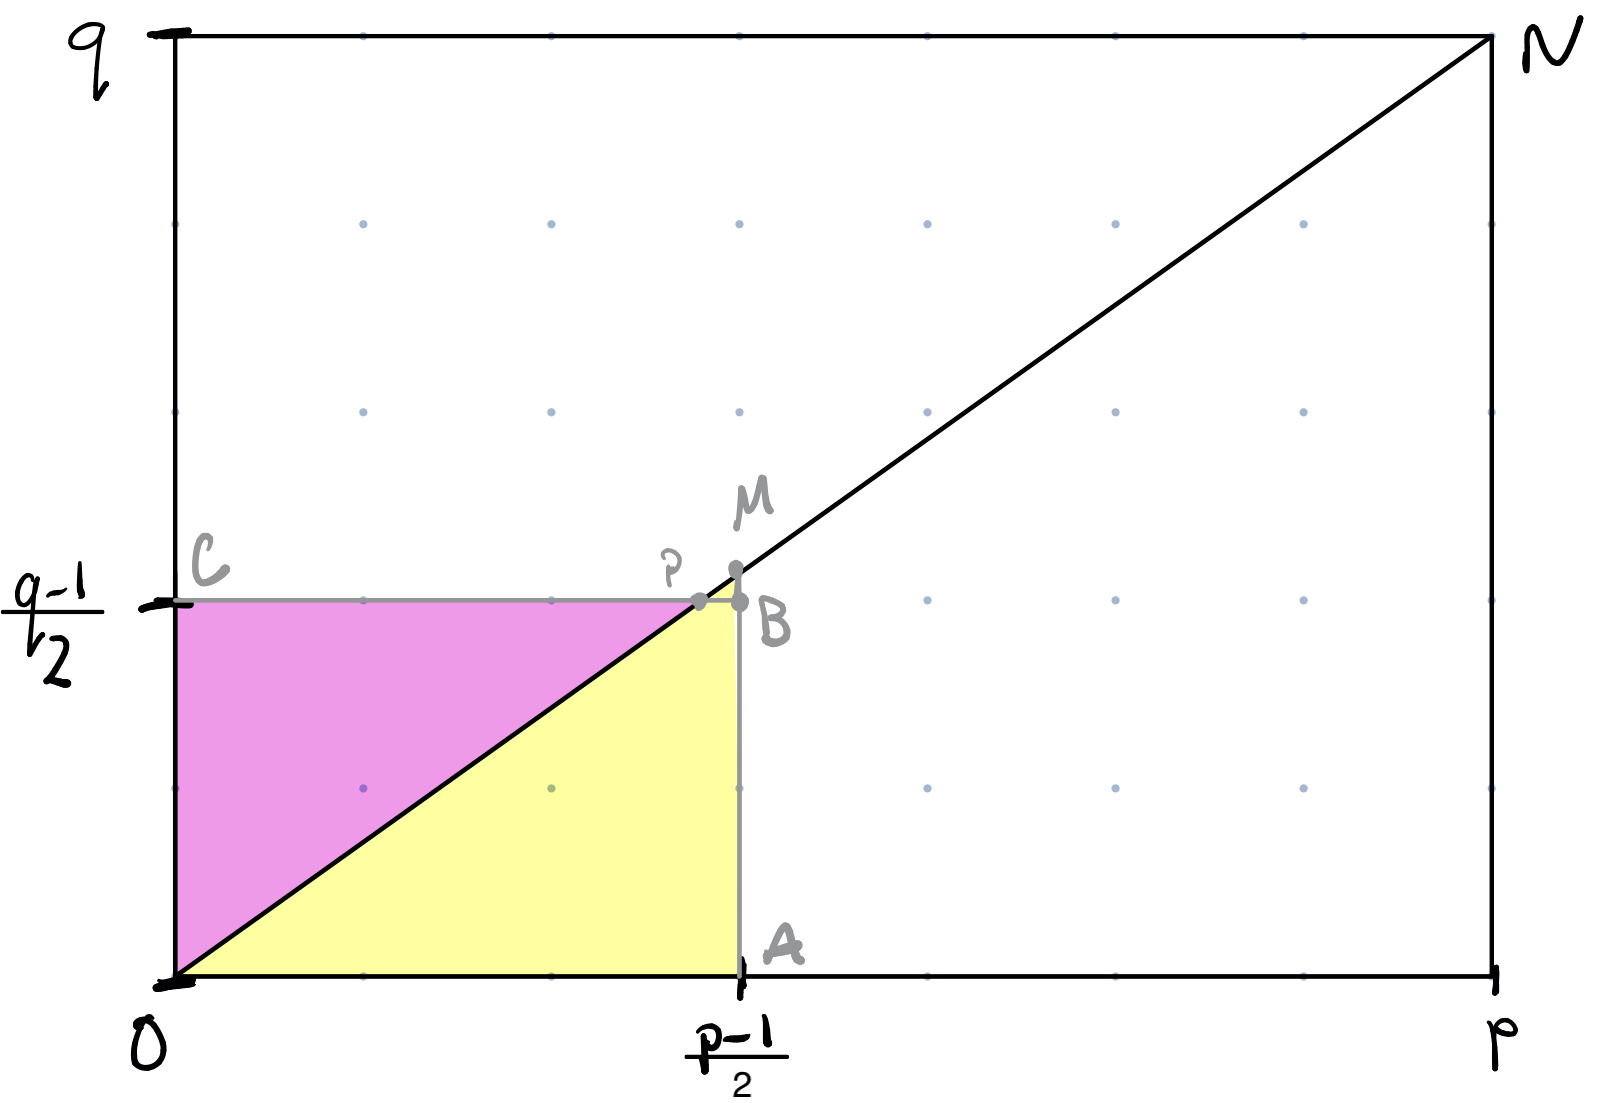
\includegraphics[width=\textwidth]{lattice}

The reading assignment was to count the lattice points in the rectangle $OABC$ outlined in grey, including those on the lines $AB$ and $BC$, but not those on $OA$ or $OC$. 

In order to count these lattice points another way, we are going to show that there are $N_1$ lattice points in the triangle $OPC$ not including $OC$(pink)  and $N_2$ lattice points in in $OAM$ not including $OA$ (yellow), thus the total number of lattice points is $N_1+N_2$. We will find that $N_1=\sum_{j=1}^{\frac{q-1}{2}}\left\lfloor\frac{jp}{q}\right\rfloor$ and $N_2=\sum_{j=1}^{\frac{-1}{2}}\left\lfloor\frac{jq}{p}\right\rfloor$. Thus, by the previous lemma, $\left\lfloor\frac{p}{q}\right\rfloor=(-1)^{N_1}$ and $\left\lfloor\frac{q}{p}\right\rfloor=(-1)^{N_2}$, which will let us finish the proof. 

We will do an examples first:

\begin{example}
 We look at the example above with $p=7$ and $q=5$.  
\begin{enumerate}[a)]
 \item The line $ON$ has slope \rule{1cm}{0.4pt}. Since $p$ and $q$ are distinct primes, there are no lattice points on $ON$ except the endpoints. 
 \item The $x$-coordinate of $M$ is \rule{1cm}{0.4pt}, $y$-coordinate of $M$ is\rule{1cm}{0.4pt}.
 \item The $y$-coordinate of $M$ lies between two consecutive integers \rule{1cm}{0.4pt} and \rule{1cm}{0.4pt}.
\end{enumerate}

Thus, the triangle $PMB$ has no lattice points except possibly those on $PB$. We can then count the number of lattice points in $OABC$ by adding the number of lattice points in $OCP$ to those in $OAM$.

To find $N_1$, the number of lattice points in $OPC$, not including those on $OC$, we count how many lattice points on the line $y=j$ are to the left of $ON$ for $j=1,2,\dots,\frac{q-1}{2}$ (in our case, this is only $j=1,2$.) Another was of saying this is for each $j$, we want the number of nonnegative integers less than 
\begin{poll} \begin{itemize}
 \item  {$\frac{7j}{5}$}
 \item {$\frac{5j}{7}$}
\end{itemize} \end{poll}

 Thus, we have for each $j$, there are 
 \begin{poll} \begin{itemize}
 \item {$\left\lfloor\frac{7j}{5}\right\rfloor$}
 \item {$\left\lfloor\frac{5j}{7}\right\rfloor$}
\end{itemize} \end{poll}
 
lattice points in $OPC$. Then $N_1=$
 \begin{poll} \begin{itemize}
 \item  {$\sum_{j=1}^{2
}\left\lfloor\frac{7j}{5}\right\rfloor$}
 \item {$\sum_{j=1}^{2
}\left\lfloor\frac{5j}{7}\right\rfloor$}
\end{itemize} \end{poll}

To find $N_2$, we use a similar counting method on $OAM$. Now, we count the lattice points on $x=j$ for $j=1,2,\dots,\frac{p-1}{2}$. Thus, for each $j$, we want the number of nonnegative integers less than \begin{poll} \begin{itemize}
 \item{$\frac{7j}{5}$}
 \item   {$\frac{5j}{7}$}
\end{itemize} \end{poll}
 Thus, we have for each $j$, there are  \begin{poll} \begin{itemize}
 \item{$\left\lfloor\frac{7j}{5}\right\rfloor$}
 \item  {$\left\lfloor\frac{5j}{7}\right\rfloor$}
\end{itemize} \end{poll}
lattice points in $OPC$. Then $N_2=$
 \begin{poll} \begin{itemize}
 \item  {$\sum_{j=1}^{3
}\left\lfloor\frac{7j}{5}\right\rfloor$}
 \item {$\sum_{j=1}^{3
}\left\lfloor\frac{5j}{7}\right\rfloor$}
\end{itemize} \end{poll}

 \end{example}
 
%\begin{ex}
%We look at the example with $p=11$ and $q=7$.  
%
% 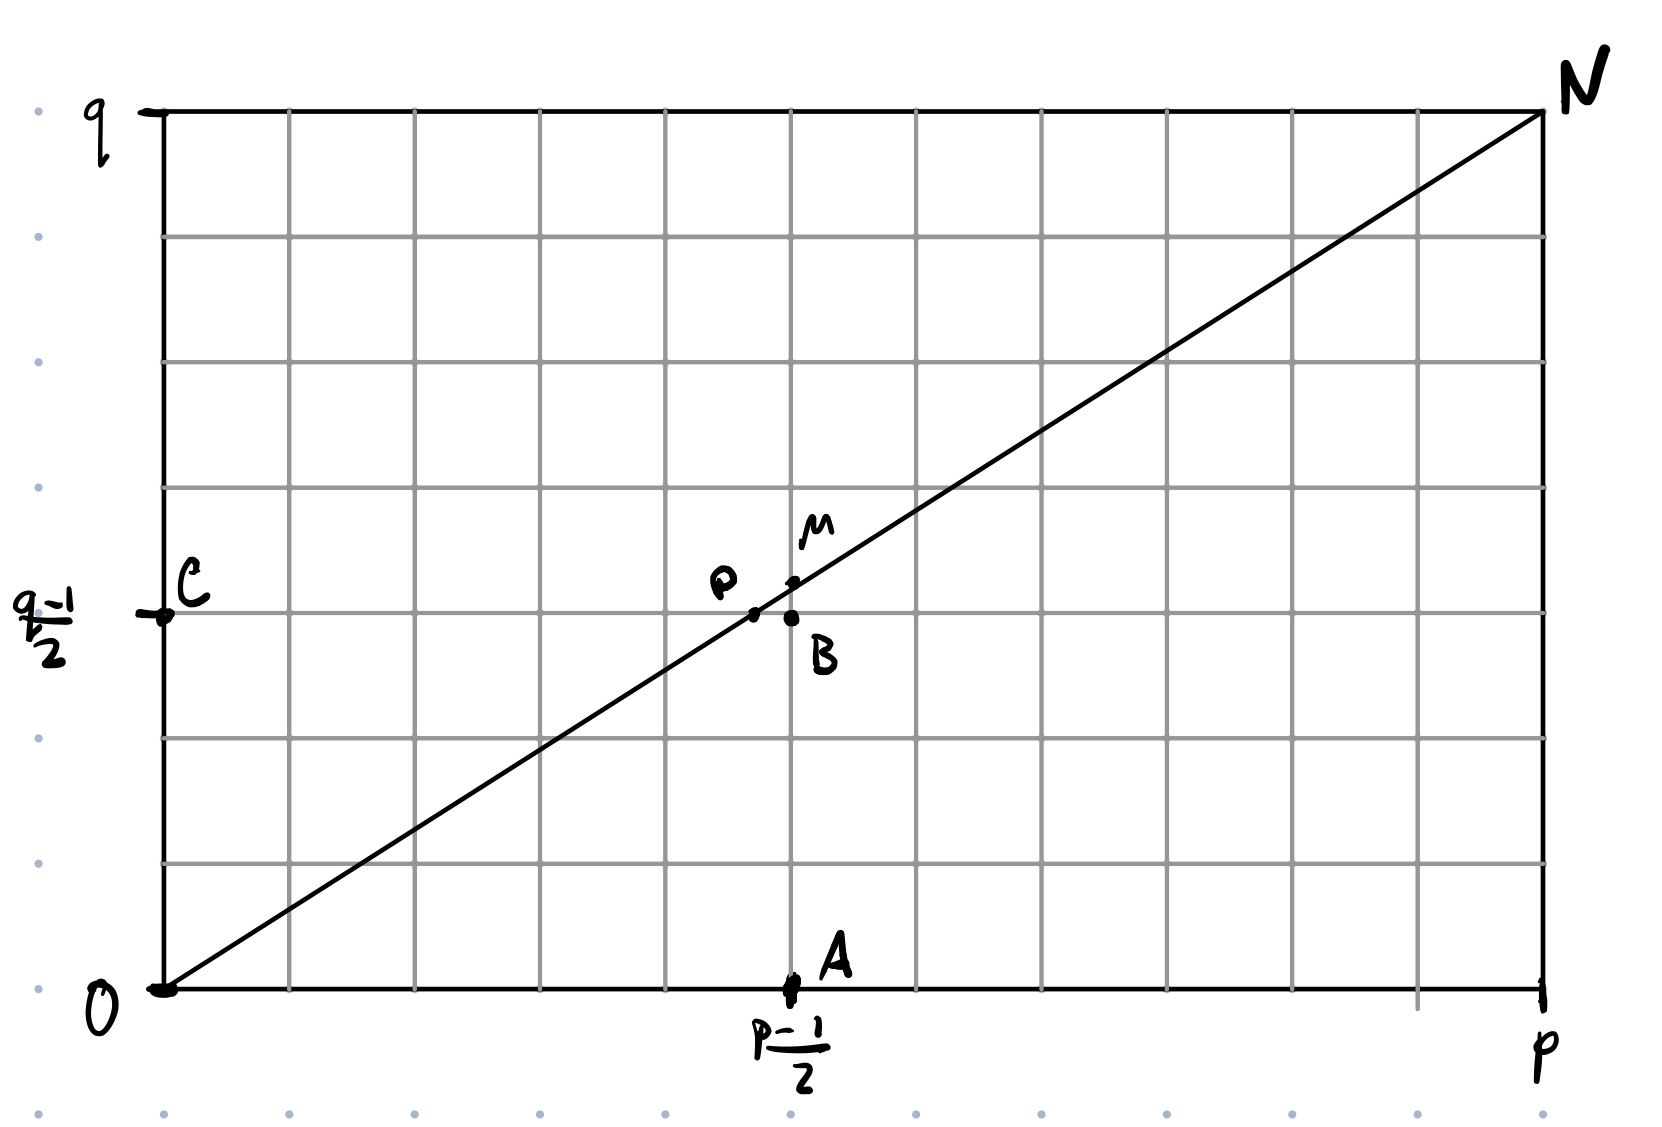
\includegraphics[width=\textwidth]{latticepoints}
%\begin{enumerate}[(a)]
% \item The line $ON$ has slope $\rule{1cm}{.4pt}{\frac{7}{11}}
% $. Since $p$ and $q$ are distinct primes, there are no lattice points on $ON$ except the endpoints. We can represent $ON$ 
% \item The $x$-coordinate of $M$ is $\rule{1cm}{.4pt}{5}
% $, $y$-coordinate of $M$ is $\rule{1cm}{.4pt}{\frac{35}{11}}
% $.
% \item The $y$-coordinate of $M$ lies between two consecutive integers $\rule{1cm}{.4pt}{3}
% $ and $\rule{1cm}{.4pt}{4}
% .$ 
%\end{enumerate}
%
%Thus, the triangle $PMB$ has no lattice points except possibly those on $PB$. We can then count the number of lattice points in $OABC$ by adding the number of lattice points in $OCP$ to those in $OAM$.
%
%To find $N_1$, the number of lattice points in $OPC$, not including those on $OC$, we count how many lattice points on the line $y=j$ are to the left of $ON$ for $j=1,2,\dots,\frac{q-1}{2}$. Another was of saying this is for each $j$, we want the number of nonnegative integers less than $j\rule{1cm}{.4pt}{\frac{11}{7}}
%$. Thus, we have for each $j$, there are $\left\lfloor j*\rule{1cm}{.4pt}{\frac{11}{7}}
%\right\rfloor$ lattice points in $OPC$. Then \[N_1=\sum_{j=1}^{\rule{1cm}{.4pt}{3}
%}\left\lfloor j*\rule{1cm}{.4pt}{\frac{11}{7}}
%\right\rfloor.\]
%
%To find $N_2$, we use a similar counting method on $OAM$. Now, we count the lattice points on $x=j$ for $j=1,2,\dots,\frac{p-1}{2}$. Thus, for each $j$, we want the number of nonnegative integers less than $j*\rule{1cm}{.4pt}{\frac{7}{11}}
%$. Thus, we have for each $j$, there are $\left\lfloor j*\rule{1cm}{.4pt}{\frac{7}{11}}
%\right\rfloor$ lattice points in $OPC$. Then \[N_2=\sum_{j=1}^{\rule{1cm}{.4pt}{5}
%}\left\lfloor j*\rule{1cm}{.4pt}{\frac{7}{11}}
%\right\rfloor.\]
%\end{ex}

Now we generalize this idea to any odd primes $p$ and $q$ with $p>q$.
\begin{enumerate}[(a)]
 \item The line $ON$ has slope $\frac{q}{p} $. Since $p$ and $q$ are distinct primes, there are no lattice points on $ON$ except the endpoints. 
  \item The $x$-coordinate of $M$ is $\frac{p-1}{2} $, $y$-coordinate of $M$ is $\frac{(p-1)}{2}\frac{q}{p}=\frac{q}{2}-\frac{q}{2p}$.
 \item The $y$-coordinate of $M$ lies between two consecutive integers $\frac{q-1}{2}$ and $\frac{q+1}{2}$, since 
\begin{align*}
 \frac{q-1}{2}&=\frac{q}{2}-\frac{1}{2}<\frac{q}{2}-\frac{q}{2p}<\frac{q}{2}<\frac{q+1}{2}
\end{align*}
\end{enumerate}

Thus, the triangle $PMB$ has no lattice points except possibly those on $PB$. We can then count the number of lattice points in $OABC$ by adding the number of lattice points in $OCP$ to those in $OAM$.


We will finish the proof Monday. \phantom\qedhere
\end{proof}
\end{document}
To find $N_1$, the number of lattice points in $OPC$, not including those on $OC$, we count how many lattice points on the line $y=j$ are to the left of $ON$ for $j=1,2,\dots,\frac{q-1}{2}$. Another was of saying this is for each $j$, we want the number of nonnegative integers less than \begin{poll} \begin{itemize}
 \item  {$\frac{jp}{q}$}
 \item {$\frac{jq}{p}$}
\end{itemize} \end{poll} 

Thus, we have for each $j$, there are 
\begin{poll} \begin{itemize}
 \item  {$\left\lfloor\frac{jp}{q}\right\rfloor$}
 \item {$\left\lfloor\frac{jq}{p}\right\rfloor$}
\end{itemize} \end{poll}
 
lattice points in $OPC$. Then $N_1=$
 \begin{poll} \begin{itemize}
 \item  {$\sum_{j=1}^{2
}\left\lfloor\frac{jp}{q}\right\rfloor$}
 \item {$\sum_{j=1}^{2
}\left\lfloor\frac{jq}{p}\right\rfloor$}
\end{itemize} \end{poll}

To find $N_2$, we use a similar counting method on $OAM$. Now, we count the lattice points on $x=j$ for $j=1,2,\dots,\frac{p-1}{2}$. Thus, for each $j$, we want the number of nonnegative integers less than  \begin{poll} \begin{itemize}
 \item {$\frac{jp}{q}$}
 \item  {$\frac{jq}{p}$}
\end{itemize} \end{poll} Thus, we have for each $j$, there are \begin{poll} \begin{itemize}
 \item{$\left\lfloor\frac{jp}{q}\right\rfloor$}
 \item   {$\left\lfloor\frac{jq}{p}\right\rfloor$}
\end{itemize} \end{poll}
lattice points in $OPC$. Then $N_2= $\begin{poll} \begin{itemize}
 \item {$\sum_{j=1}^{2
}\left\lfloor\frac{jp}{q}\right\rfloor$}
 \item  {$\sum_{j=1}^{2
}\left\lfloor\frac{jq}{p}\right\rfloor$}
\end{itemize} \end{poll}
From the previous Lemma, $\left(\frac{p}{q}\right)=(-1)^{N_1}$ and $\left(\frac{q}{p}\right)=(-1)^{N_2}$. Thus, 
\begin{align*}
 \left(\frac{p}{q}\right)\left(\frac{p}{q}\right)&=(-1)^{N_1} (-1)^{N_2} \\
 &=(-1)^{N_1+N_2}\\
&=(-1)^{\frac{p-1}{2}\frac{q-1}{2}}
\end{align*}
with the result from the participation assignment.
\end{proof}

Quadratic reciprocity means that determining all quadratic residues (perfect squares) modulo an odd prime is a finite problem. In terms of Legendre symbol, this is finding all $a$ where $\left(\frac{a}{p}\right)=1$ for a given $p$. For example, when $p=11$, we can check all positive integers $a$. However, what about the reverse? Quadratic reciprocity allows us to find all odd primes $p$ where $\left(\frac{11}{p}\right)=1,$ even though there are infinitely many odd primes. This idea is also on Homework 12, Short Proofs.


%%%%%%%%%%%%%%%%%%%%%%%%%
\subsection{Announcements (5 min)}
%%%%%%%%%%%%%%%%%%%%%%%%%
We are going to leave quadratic reciprocity for nonprimes for independent study. Hopefully, if you need this information in the future, you have gained some of the skill of reading and working through mathematics. 

In the interest of moving away from super technical topics, we are going to skip arithmetic functions and the M\"obius inversion formula. This will make the last week a bit of a grab bag of number theory topics, but I want to move into Diophantine equations, which are more concrete. This will also keep us looking at things that are vaguely geometric.

We also are going to take a slightly different approach than the book, and use Pythagorean triples as our motivating example. This means we will do parts of Chapter 11 before Chapter 10.


%%%%%%%%%%%%%%%%%%%%%%%%%%
\subsection{Linear Diophantine equation review (10 minutes)}
%%%%%%%%%%%%%%%%%%%%%%%%%%

\begin{defn}
 A \emph{Diophantine equation} is any equation in one or more variables to be solved in the integers.
\end{defn}
\begin{defn}
 Let $a_1,a_2,\dots,a_n,b\in\mathbb{Z}$ with $a_1,a_2,\dots,a_n$ not zero. A Diophantine equation of the form \[a_1x_1+a_2x_2+\cdots+a_nx_n=b\] is a \emph{linear Diophantine equation in the $n$ variable $x_1,\dots,x_n$}.
\end{defn}

The participation assignment classifies linear Diophantine equations in one variable.

The question of whether there are solutions to Diophantine equations becomes harder when there is more than one variable. Then next step is to classify Diophantine equations in two variables.

\begin{thm}[Theorem 1.13]
 Let $ax+by=c$ be a linear Diophantine equation in the variables $x$ and $y$. Let $d=(a,b)$. If $d\nmid c$, then the equation has no solutions; if $d\mid c$, then the equation has infinitely many solutions. Furthermore, if $x_0,y_0$ is a particular solution of the equation, then all solution are given by $x=x_0+\frac{b}{d}n$ and $y=y_0-\frac{a}{d}n$ where $n\in\mathbb{Z}$.
\end{thm}
\begin{br}
Find all solutions to $803x+154y=11$.
\end{br}
%Using the Euclidean Algorithm, we find:
% 
%\begin{align*}
% 803&=154*\rule{1cm}{.4pt}+\rule{1cm}{.4pt}\\
% 154&=\rule{1cm}{.4pt}*\rule{1cm}{.4pt}+\rule{1cm}{.4pt}\\
%\rule{1cm}{.4pt}&=\rule{1cm}{.4pt}*1+\rule{1cm}{.4pt}
%\end{align*}
%Thus
%\begin{align*}
% (803,154)&=\rule{1cm}{.4pt}-\rule{1cm}{.4pt}\\
% &=\rule{1cm}{.4pt}-(154-\rule{1cm}{.4pt}*\rule{1cm}{.4pt})=\rule{1cm}{.4pt}*\rule{1cm}{.4pt}-154\\
% &=(803-154*\rule{1cm}{.4pt})*\rule{1cm}{.4pt}-154=803*\rule{1cm}{.4pt}{5}-154*\rule{1cm}{.4pt}{26}
%\end{align*}
%
%Thus, all solutions to the Diophantine equation have the form $x=\rule{1cm}{.4pt}{5}+\frac{\rule{1cm}{.4pt}{154}}{\rule{1cm}{.4pt}{11}}n$ and $y=\rule{1cm}{.4pt}{-26}-\frac{\rule{1cm}{.4pt}{803}}{\rule{1cm}{.4pt}{11}}n$.


%\begin{example}
% There is a famous riddle about Diophantus: ``God gave him his boyhood one-sixth of his life, One twelfth more as youth while whiskers grew rife; And then yet one-seventh ere marriage begun; In five years there came a bouncing new son. Alas, the dear child of master and sage After attaining half the measure of his father's life chill fate took him. After consoling his fate by the science of numbers for four years, he ended his life." 
% 
% That is: Diophantus's childhood was $1/6^{th}$ of his life, adolescence was $1/12^{th}$ of his life, after another $1/7^{th}$ of his life he married, his son was born 5 years after he married, his son then died at half the age that Diophantus died, and 4 years later Diophantus died.
% 
%The Diophantine equation that let's us solve this riddle is: \[x=\frac{x}{6}+\frac{x}{12}+\frac{x}{7}+5+\frac{x}{2}+4.\] Then, Diophantus's childhood was $\rule{1cm}{.4pt}{14}$ years, his adolescence was $\rule{1cm}{.4pt}{7}$ years, he married when he was $\rule{1cm}{.4pt}{33}$, his son was born when he was $\rule{1cm}{.4pt}{38}$ and died $\rule{1cm}{.4pt}{42}$ years later, then Diophantus died when he was $\rule{1cm}{.4pt}{84}$.
%\end{example}

%%%%%%%%%%%%%%%%%%%%%%%%%%
\subsection{Nonlinear Diophantine equations}
%%%%%%%%%%%%%%%%%%%%%%%%%%
\begin{defn}
 A Diophantine equation is \emph{nonlinear} if it is not linear.
\end{defn}

\begin{example}
 
\begin{enumerate}
 \item The Diophantine equation $x^2+y^2=z^2$ is our next section. Solutions are called Pythagorean triples.
 \item Let $n\in\mathbb{Z}$ with $n\geq 3$. The Diophantine equation $x^n+y^n=z^n$ is the subject of the famous Fermat's Last Theorem. We will also prove one case of this.
 \item Let $n\in\mathbb{Z}$. The Diophantine equation $x^2+y^2=n$ tells us which integers can be represented as the sum of two squares.
 \item Let $d,n\in\mathbb{Z}$. The Diophantine equation $x^2-dy^2=n$ is known as Pell's equation.
\end{enumerate}
\end{example}

Sometimes we can use congruences to show that a particular nonlinear Diophantine equation has no solutions. 

\begin{example}
 Prove that $3x^2+2=y^2$ is not solvable.
 
 Assume that there is a solution. Then any solution to the Diophantine equation is also a solution to the congruence $3x^2+2\equiv y^2 \mod 3$, which implies $2\equiv y^2 \mod 3$, which we know is false. Thus there are no integer solutions to $3x^2+2=y^2$.
\end{example}

Note: viewing the same equation modulo 2 says $x^2\equiv y^2 \mod 2$, which does not give us enough information to prove a solution does not exist.
%%%%%%%%%%%%%%%%%%%%%%%%%%
\subsection{Pythagorean triples}
%%%%%%%%%%%%%%%%%%%%%%%%%%
One of the most famous math equations is $x^2+y^2=z^2$, probably because we learn it in high school. We are going to classify all integer solutions to the equation.

\begin{defn}
 A triple $(x,y,z)$ of positive integers satisfying the Diophantine equation $x^2+y^2=z^2$ is called \emph{Pythagorean triple}.
\end{defn}

 Select the Pythagorean triples:
 \begin{poll}
\begin{itemize}
  \item  {3,4,5}
 \item {5,12,13}
 \item{-3,4,5}
 \item {6,8,10}
 \item{0,1,1}
\end{itemize}
\end{poll}



It is actually possible to classify all Pythagorean triples, just like we did for linear Diophantine equations in two variables. To simplify this process, we will work with $x,y,z>0$, and $(x,y,z)=1$. For any given solution of this form, we have that $(-x,y,z),(x,-y,z),(x,y,-z),(-x,-y,z),(x,-y,-z),(-x,y,-z),$ and $(-x,-y,-z)$ are also solutions to the Diophantine equation, as is $(nx,ny,nz)$ for any integer $n$. Thus, we call such a solution a \emph{primitive Pythagorean triple}.  We call $(0,n,\pm n)$ and $(n,0,\pm n)$ the \emph{trival solutions}.

\begin{thm}
For a primitive Pythagorean triple $(x,y,z)$, exactly one of $x$ and $y$ is even.
\end{thm}
\begin{proof}
 If $x$ and $y$ are both even, then $z$ must also be even, contradicting that $(x,y,z)=1$.
 
 If $x$ and $y$ are both odd, then $z$ is even. Now we can work modulo $4$ to get a contradiction. Since $x$ and $y$ are odd, we have that $x^2\equiv y^2\equiv \rule{1cm}{.4pt}\pmod 4$. Since $z$ is even, we have that $z^2\equiv \rule{1cm}{.4pt}\pmod 4$, but $x^2+y^2\equiv \rule{1cm}{.4pt}\pmod 4$.
 
 Thus, the only remaining option is exactly one of $x$ and $y$ is even.
\end{proof}

\end{document}